% Combined Report — Condensate Partition Coefficient Pipeline
% Black ink only (no color). Compile with pdfLaTeX (e.g. upload this folder to
% Overleaf and press Recompile). Figures are expected in ./figures.
\documentclass[11pt]{article}
\usepackage[margin=1in]{geometry}
\usepackage{amsmath}
\usepackage{mathptmx}            % Times serif — clean, no color
\usepackage[T1]{fontenc}
\usepackage{graphicx}
\usepackage{booktabs}
\usepackage{longtable}
\usepackage{array}
\usepackage{ragged2e}
\usepackage{titlesec}
\usepackage{fancyhdr}
\usepackage[hidelinks]{hyperref}
\graphicspath{{figures/}}

\titleformat{\section}{\Large\bfseries}{\thesection}{0.6em}{}
\titleformat{\subsection}{\large\bfseries}{\thesubsection}{0.6em}{}
\titleformat{\subsubsection}{\normalsize\bfseries}{}{0em}{}
\setlength{\parskip}{0.5em}
\setlength{\parindent}{0pt}
\setlength{\emergencystretch}{3em}   % absorb long unbreakable code tokens in justified text
\newcommand{\code}[1]{\texttt{\small #1}}

\pagestyle{fancy}\fancyhf{}
\lhead{\small Condensate Partition Coefficient Pipeline}
\rhead{\small Franco Lab \textbullet\ UCLA}
\cfoot{\small\thepage}
\renewcommand{\headrulewidth}{0.4pt}

\begin{document}

% ── Title page ────────────────────────────────────────────────────────────────
\begin{titlepage}
\centering
\vspace*{3cm}
{\Huge\bfseries Condensate Partition\\[0.3em] Coefficient Pipeline\par}
\vspace{1cm}
{\LARGE Combined Report\par}
\vspace{0.5cm}
{\large User Manual \quad\textbullet\quad Methods \quad\textbullet\quad Research Timeline \quad\textbullet\quad JABr Reference Data\par}
\vfill
{\large\bfseries Franco Lab \textbullet\ University of California, Los Angeles\par}
\vspace{0.4cm}
{\large Author: Daniel Chang\par}
{\large Principal Investigator: Elisa Franco\par}
\vspace{0.8cm}
{Spring 2026\par}
\end{titlepage}

\tableofcontents
\newpage

\section{Part I --- User Manual}

This pipeline replaces the manual Imaris workflow for measuring the partition
coefficient (PC) of nuclear biomolecular condensates. Given a two-channel confocal
Z-stack (channel 0 = nuclei, channel 1 = condensate), it segments nuclei and
condensates in 3D, computes the PC, and reports a calibrated value on the manual
reference scale. It runs from a point-and-click graphical interface or the command line.

\begin{center}
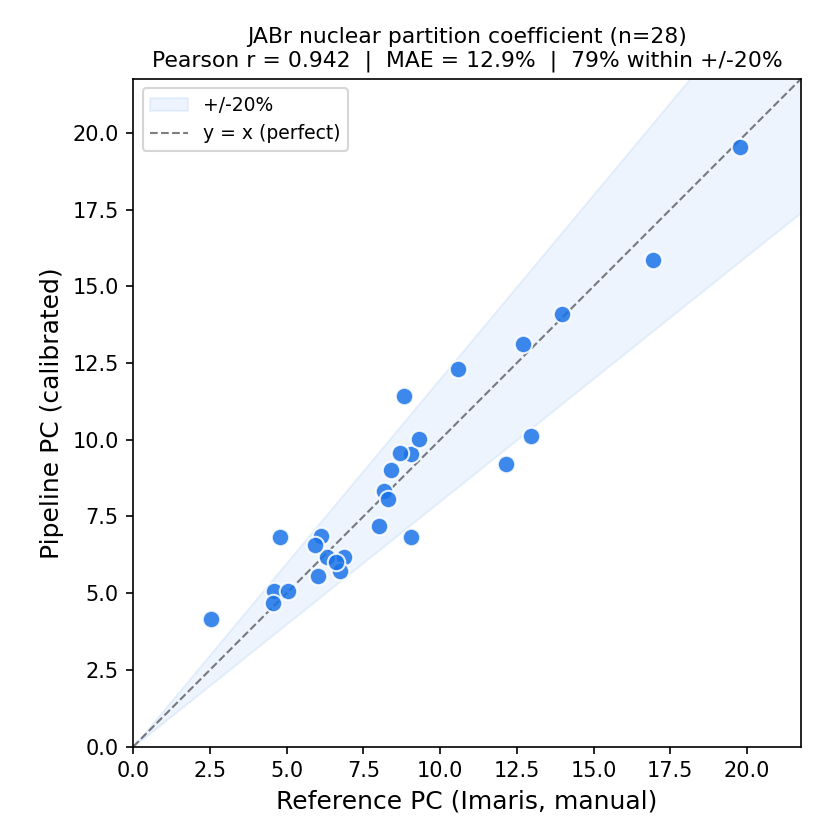
\includegraphics[width=0.6\textwidth]{jabr_validation.png}\\
{\small Validation on JABr: calibrated pipeline PC vs the manual Imaris reference.}
\end{center}

\subsection{Installation (one time)}
Install Python 3.10 or 3.11, then install PyTorch for your machine (CPU or your CUDA
version) from \href{https://pytorch.org/get-started/locally/}{pytorch.org}. Example for CUDA 12.1:
\begin{quote}\ttfamily\small pip install torch -{}-index-url\\ \hspace*{1.5em}https://download.pytorch.org/whl/cu121\end{quote}
Then install the remaining dependencies:
\begin{quote}\code{pip install -r requirements.txt}\end{quote}
On first run, Cellpose downloads its model weights automatically (one-time
$\sim$100\,MB). A GPU is recommended ($\sim$10--15\,s per cell); CPU works but is slower.

\subsection{Preparing image files}
The pipeline accepts either one multi-channel TIF (both channels in one file) or two
separate single-channel TIFs. \textbf{Channel order matters:} channel 0 must be nuclei,
channel 1 the condensate. Most axis orderings (ZCYX, CZYX, \dots) are auto-detected; if
results look wrong, swapped channels are the most common cause.

\subsection{Running with the graphical interface}
Launch with \code{python run\_gui.py}. A window with \textbf{Single File} and \textbf{Batch}
tabs opens.
\begin{enumerate}\setlength{\itemsep}{1pt}
\item On the \textbf{Single File} tab, choose the input mode and browse to your data.
\item Choose an output folder (optional).
\item In \textbf{Settings}, set \textbf{Construct = JABr}; leave all other settings at their defaults.
\item Click \textbf{Run Pipeline}. Progress streams in the Output Log; the status reads \textbf{Done} when finished.
\item Open your output folder for the masks, tables, and \code{results.png}.
\end{enumerate}

\subsection{Settings}
For routine JABr analysis you only need to set \textbf{Construct}; the rest have sensible defaults.

\begin{center}
\renewcommand{\arraystretch}{1.2}
\begin{tabular}{>{\RaggedRight}p{3.2cm} >{\RaggedRight}p{1.5cm} >{\RaggedRight}p{8.3cm}}
\toprule
\textbf{Setting} & \textbf{Default} & \textbf{What it does}\\
\midrule
Construct & (none) & Pick JABr for the validated workflow. Auto-selects the \code{blob\_log} detector and the JABr calibration so the reported PC is on the manual scale.\\
Condensate detector & auto & \code{auto} routes JABr to \code{blob\_log}, else Cellpose. Normally left on auto.\\
Top-X\% brightest & 75 & Defines condensed-phase density; trims the dim mask halo to match the manual reference. Leave at 75.\\
Nuclei cell-prob. & $-2.0$ & How aggressively nuclei are detected. $-2.0$ suits the lab's nuclear stain.\\
blob\_log threshold & 0.03 & Condensate spot sensitivity (used when detector = \code{blob\_log}). Leave at 0.03 for JABr.\\
Disable GPU & off & Tick on a laptop with no NVIDIA GPU.\\
\bottomrule
\end{tabular}
\end{center}
\textbf{The one rule for routine use:} set Construct = JABr and run.

\subsection{Reading the outputs}
Every run writes \code{summary.csv} (headline numbers including the calibrated PC),
\code{results.png}, \code{condensate\_masks.tif} and \code{nuclei\_masks.tif} (3D labeled
masks), and per-object/per-slice CSVs. For the bundled sample \code{JABr\_Sample2\_5\_3.tif},
a real run produces nuclear PC raw 4.867 calibrated to 4.813 (manual reference 4.558,
$+5.6\%$). Report the calibrated nuclear PC, and always glance at \code{condensate\_masks.tif}
over the raw channel in Fiji/ImageJ to catch the rare misfire.

\begin{center}
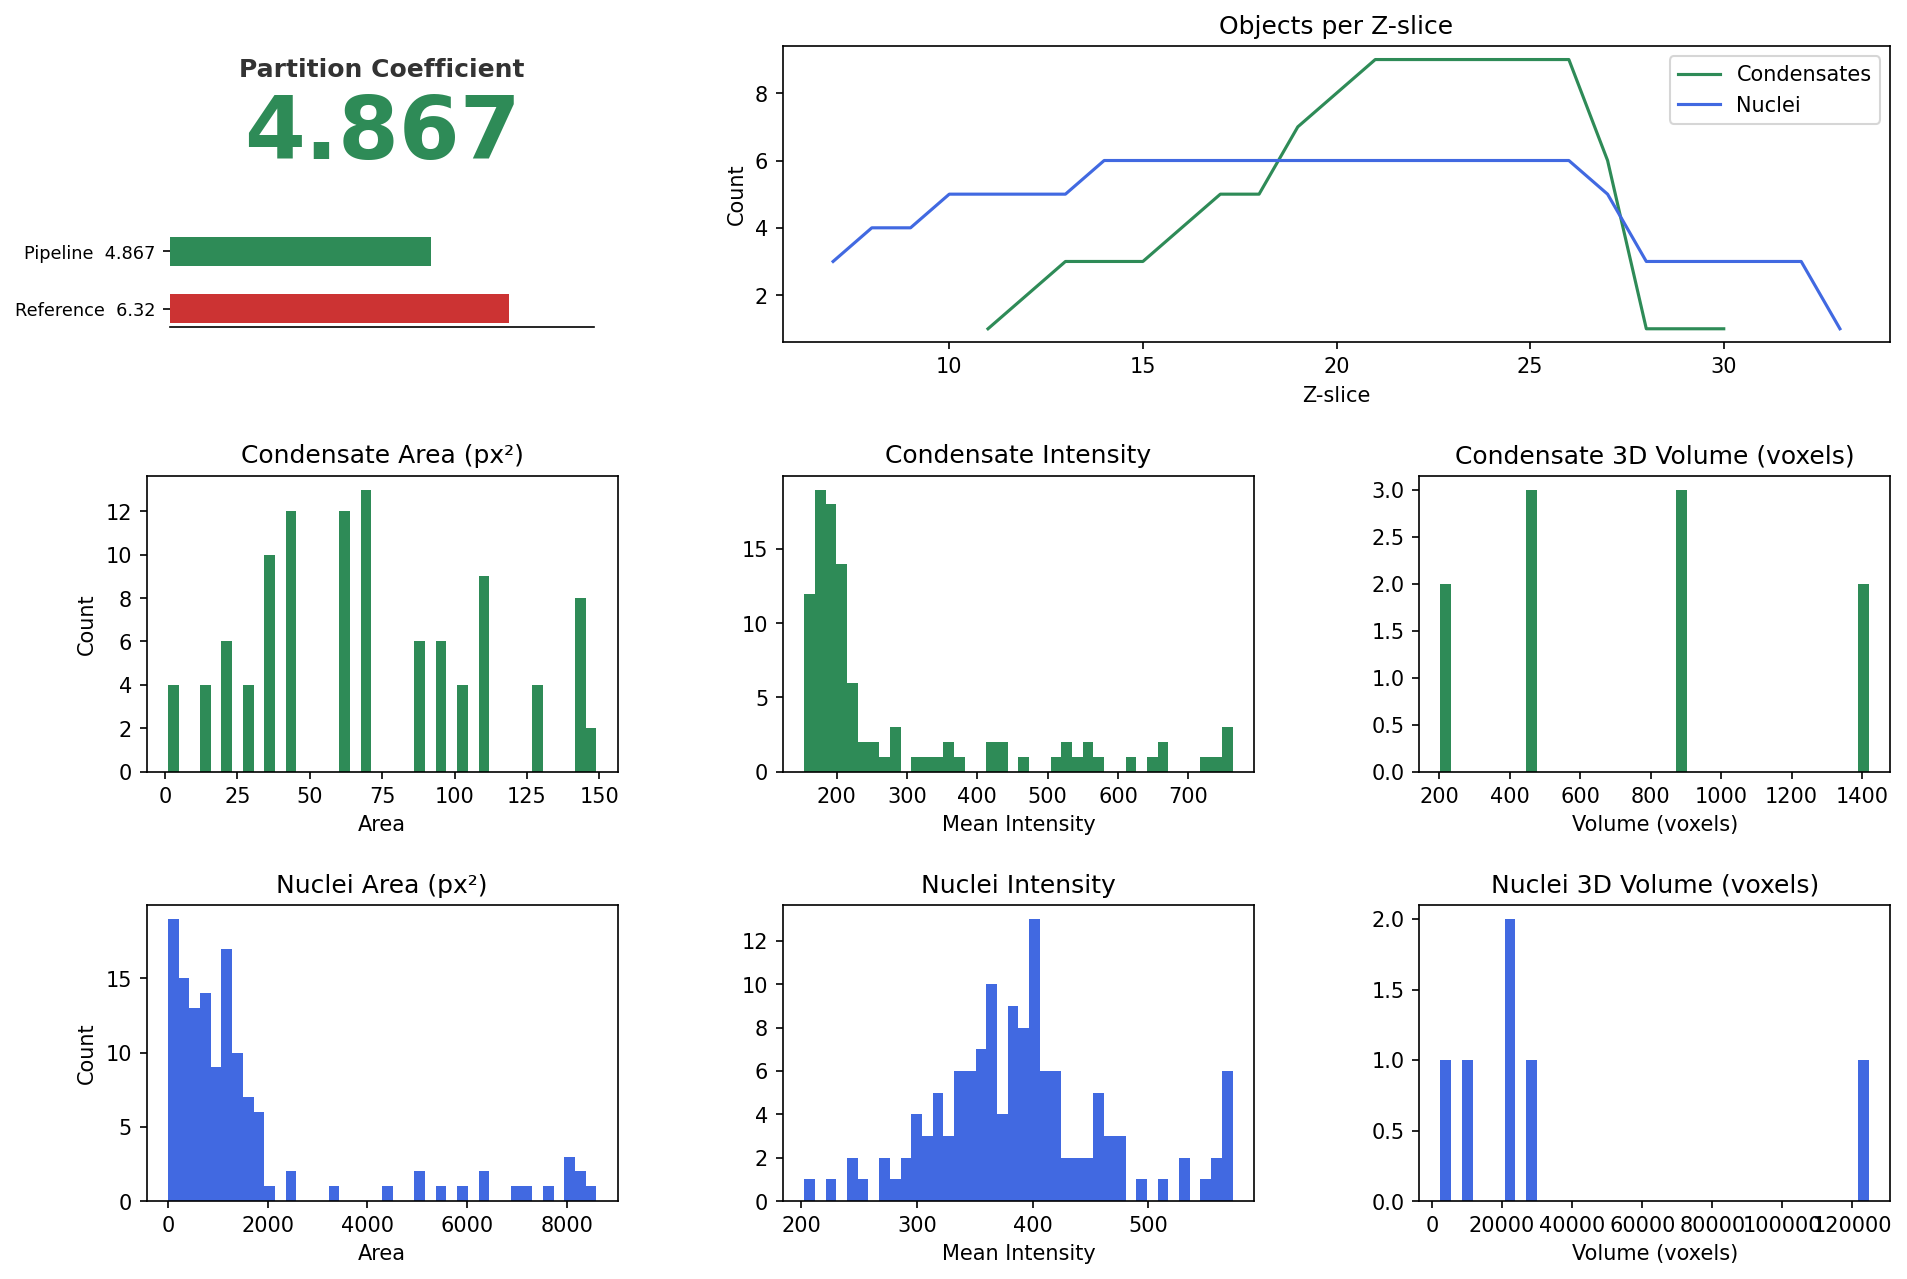
\includegraphics[width=0.95\textwidth]{example_results.png}\\
{\small \code{results.png} from the bundled-sample run.}
\end{center}

\subsection{Command line}
\begin{quote}\ttfamily\small python pipeline.py -{}-roi sample\_data/JABr\_Sample2\_5\_3.tif\\ \hspace*{1.5em}-{}-construct JABr -{}-output my\_output\end{quote}
Separate channels: \code{-{}-nuc nuclei.tif -{}-cond condensate.tif}. Physical volumes in
$\mu m^3$: add \code{-{}-voxel-xy 0.065 -{}-voxel-z 0.3}. Force CPU: \code{-{}-no-gpu}. For
many files (and optional comparison vs a manual reference CSV), use the GUI \textbf{Batch} tab.

\subsection{Troubleshooting}
\begin{center}
\begin{tabular}{>{\RaggedRight}p{5cm} >{\RaggedRight}p{8cm}}
\toprule
\textbf{Symptom} & \textbf{Likely cause / fix}\\
\midrule
PC wildly off / nuclei empty & Channels swapped: confirm ch0 = nuclei, ch1 = condensate.\\
``0 condensates detected'' & Not JABr, or very dim signal. Lower \code{blob\_log} threshold (e.g.\ 0.02).\\
Very slow (minutes/cell) & Running on CPU. Install a CUDA PyTorch build; ensure Disable GPU is unchecked.\\
\code{CUDA out of memory} & Tick Disable GPU, or close other GPU programs.\\
One cell's calibrated PC off & Calibration is population-level; cells vary ($\pm 20\%$ for $\sim$80\% of cells).\\
\bottomrule
\end{tabular}
\end{center}
\newpage

\section{Part II --- Methods}

\subsection{The quantity}
The partition coefficient is PC = condensed-phase density / dilute-phase density
(Fabrini et al.). All intensities are background-subtracted, where the background $B$
is the minimum voxel intensity across the field of view (camera offset).
\begin{itemize}\setlength{\itemsep}{1pt}
\item \textbf{Condensed-phase density} --- mean of $\mathrm{clip}(\text{intensity}-B,0)$
over the brightest 75\% of voxels inside both a condensate mask and a nucleus. Automated
masks include a dim halo a manual tracing would exclude; trimming the bottom 25\% recovers
densities consistent with the manual reference.
\item \textbf{Dilute-phase density} --- mean of the 50 lowest-intensity valid
$10\times10\times10$-voxel patches inside the nuclear dilute region. Averaging many low
patches approximates a manual quiet-region selection and is far more stable than a single random patch.
\end{itemize}

\subsection{Pipeline steps}
\begin{center}
\begin{tabular}{>{\RaggedRight}p{2.4cm} >{\RaggedRight}p{4.6cm} >{\RaggedRight}p{6cm}}
\toprule
\textbf{Step} & \textbf{Method} & \textbf{Why}\\
\midrule
Denoise & Cellpose 3 \code{denoise\_cyto3} per slice & Removes shot noise; PC intensities are read from the raw stack.\\
Segment nuclei & Cellpose 3 \code{cyto3}, \code{do\_3D} & Native 3D nuclear segmentation.\\
Clean nuclei & Connected-component relabel; drop $<1000$-voxel fragments & Cellpose over-splits large nuclei; relabeling restores whole nuclei.\\
Fill voids & Per-nucleus \code{binary\_fill\_holes} (3D + 2D) & Condensates carve donut holes in the nuclear stain exactly where nuclear condensates sit; filling makes them count as intra-nuclear.\\
Detect condensates & \code{blob\_log} (LoG), $\sigma$ 1.5--6.0, threshold 0.03 & Classical, parameter-light detector matched to roughly-spherical condensates; each rendered as a sphere of radius $\sigma\sqrt{3}$.\\
Intra-nuclear gate & Keep a blob if $\geq 50\%$ of its sphere lies inside a nucleus & Replaces an older single-centroid test that mis-handled boundary blobs and crowded fields.\\
Calibrate & Per-construct linear (JABr) / isotonic map & Standardizes the automated PC onto the manual Imaris scale.\\
\bottomrule
\end{tabular}
\end{center}

\subsection{Why there is a calibration}
The automated and manual workflows define the condensed and dilute regions slightly
differently: the automated condensed region runs brighter (brightest mask voxels) and the
automated dilute region runs dimmer (quietest sampled patches) than a hand-drawn Imaris
region. Both push the ratio the same way, so the raw automated PC is systematically about
$3\times$ the manual reference --- but consistently so ($r = 0.94$). A single linear map converts it back:
\begin{quote}\code{calibrated\_PC = 0.3642 * raw\_PC + 3.0405}\quad (JABr)\end{quote}
This is cross-method standardization, not a fudge factor. A linear map is rank-preserving,
so calibration cannot improve correlation --- it only removes the scale/offset bias. The
correlation $r$ is therefore the true accuracy ceiling, and calibration is meaningful only where $r$ is already high.

\subsection{Scope and generalization}
The pipeline is validated and production-ready for JABr. It is construct-specific: the
\code{blob\_log} parameters encode JABr's condensate size and brightness and do not transfer
unchanged. Cross-construct correlation vs Imaris:
\begin{center}
\begin{tabular}{l c >{\RaggedRight}p{7cm}}
\toprule
\textbf{Construct} & \textbf{Pearson r} & \textbf{Status}\\
\midrule
JABr & 0.942 & Production\\
GABr & 0.678 & Mediocre; isotonic calibration, use with caution\\
AABr & 0.122 & Not usable as-is\\
AwtBr & $-0.116$ & Not usable as-is\\
GwtBr & $-0.341$ & Not usable as-is\\
\bottomrule
\end{tabular}
\end{center}
A leave-one-construct-out test (a single learned Cellpose detector, evaluated on a construct
it never trained on) confirmed that one model does not generalize zero-shot: it fails by
under-detection, staying silent on most cells of an unseen construct. The route to extend the
tool is per-construct calibration where correlation is already acceptable, or few-shot
retraining with a handful of labeled ROIs of the new construct --- far cheaper than a manual parameter sweep.
\newpage

\section{Part III --- Research Timeline}
A chronological record of how the pipeline was built. Dates are from the project's version-control history.

\subsection*{Winter 2026 --- Foundation}
\begin{center}
\begin{tabular}{>{\RaggedRight}p{2cm} >{\RaggedRight}p{11.5cm}}
\toprule
\textbf{Date} & \textbf{Milestone}\\
\midrule
2026-03-17 & Initial clean pipeline established. \\
2026-03-24 & Winter 2026 report finalized; baseline segmentation + PC concept. \\
\bottomrule
\end{tabular}
\end{center}
\subsection*{April 2026 --- Segmentation survey \& the PC formula}
\begin{center}
\begin{tabular}{>{\RaggedRight}p{2cm} >{\RaggedRight}p{11.5cm}}
\toprule
\textbf{Date} & \textbf{Milestone}\\
\midrule
2026-04-22 & Spring segmentation-model survey; 4 candidate models compared. \\
2026-04-25 & Background-subtracted PC formula adopted across all scripts. \\
2026-04-30 & PC now matches reference: connected-component nuclei fix + lowest-patch dilute density; 50-patch stability fix. \\
\bottomrule
\end{tabular}
\end{center}
\subsection*{May 2026 --- Calibration, GUI, generalization}
\begin{center}
\begin{tabular}{>{\RaggedRight}p{2cm} >{\RaggedRight}p{11.5cm}}
\toprule
\textbf{Date} & \textbf{Milestone}\\
\midrule
2026-05-06 & Batch cross-reference pipeline; top-75\% condensate-density calibration. \\
2026-05-07 & GUI built; laptop (CPU) validation; PI meeting. \\
2026-05-14 & Crowded-field debugging; max-overlap-nucleus target-cell heuristic. \\
2026-05-16 & First fine-tuned Cellpose model; 5-construct accuracy sweep; per-construct calibration. \\
2026-05-18 & M187 research poster (PC = 6.297 vs 6.32 reference). \\
2026-05-28 & blob\_log detector wired into the pipeline; JABr calibration refit; GUI gains construct/detector controls; cytoplasmic PC added. \\
\bottomrule
\end{tabular}
\end{center}
\subsection*{June 2026 --- Production hardening \& honest scope}
\begin{center}
\begin{tabular}{>{\RaggedRight}p{2cm} >{\RaggedRight}p{11.5cm}}
\toprule
\textbf{Date} & \textbf{Milestone}\\
\midrule
2026-06-10 & Discussion section; nuclei void-filling so condensates in donut holes count toward the PC. \\
2026-06-11 & Sphere-overlap intra-nuclear gate promoted to production: JABr r 0.926 to 0.942, MAE 14.6\% to 13.7\%. \\
2026-06-12 & Leave-one-construct-out experiment: a single learned detector does not generalize zero-shot. Few-shot path mapped. \\
2026-06-13 & Clean public release: repository, instruction manual, methods writeup, and this combined report. \\
\bottomrule
\end{tabular}
\end{center}
\subsection*{Where it stands}
Validated, production-ready for JABr ($r = 0.942$, MAE 12.9\%, 79\% of cells within
$\pm 20\%$, n = 28). Delivered: a CLI, a GUI for non-coding lab use, per-construct
calibration, and full documentation. Known boundary, with a plan: the detector is
JABr-specific; extending it needs per-construct calibration or few-shot retraining.
\newpage

\section{Part IV --- JABr Reference Data}
Source: Box \textrightarrow\ Condensate Volume Quantification \textrightarrow\ JABr. The
manual Imaris measurements (nuclear and cytoplasmic) are the ground truth against which the
pipeline is validated; the pipeline results table is the production \code{blob\_log} V4 output
(sphere-overlap gate, linear calibration).

\subsection*{Manual reference --- Nuclear (n = 30)}
\begin{center}
\begin{longtable}{l r r r}
\toprule
\textbf{File} & \textbf{Condensate Density} & \textbf{Dilute Density} & \textbf{Partition Coefficient} \\
\midrule
\endfirsthead
\toprule
\textbf{File} & \textbf{Condensate Density} & \textbf{Dilute Density} & \textbf{Partition Coefficient} \\
\midrule
\endhead
\bottomrule
\endlastfoot
Sample1\_1\_1 & 390.42 & 81.67 & 4.780 \\
Sample1\_1\_2 & 827.87 & 91.60 & 9.038 \\
Sample1\_1\_3 & 1516.55 & 76.69 & 19.774 \\
Sample1\_1\_4 & 793.32 & 74.96 & 10.584 \\
Sample1\_2\_1 & 619.05 & 77.16 & 8.023 \\
Sample1\_2\_2 & 339.36 & 73.78 & 4.599 \\
Sample1\_2\_3 & 162.87 & 63.99 & 2.545 \\
Sample1\_4\_1 & 540.60 & 88.20 & 6.129 \\
Sample1\_4\_2 & 368.83 & 73.05 & 5.049 \\
Sample1\_4\_3 & 1338.28 & 95.84 & 13.963 \\
Sample1\_4\_4 & 584.31 & 62.68 & 9.322 \\
Sample2\_5\_1 & 658.30 & 104.09 & 6.324 \\
Sample2\_5\_2 & 483.19 & 70.30 & 6.873 \\
Sample2\_5\_3 & 331.24 & 72.67 & 4.558 \\
Sample2\_5\_4 & 415.30 & 68.99 & 6.020 \\
Sample2\_5\_5 & 497.00 & 73.88 & 6.728 \\
Sample2\_5\_6 & 894.09 & 73.58 & 12.151 \\
Sample3\_3\_1 & 534.27 & 65.28 & 8.185 \\
Sample3\_3\_2 & 633.55 & 70.04 & 9.045 \\
Sample3\_3\_3 & 788.77 & 89.38 & 8.825 \\
Sample3\_3\_4 & 481.04 & 72.90 & 6.599 \\
Sample3\_3\_5 & 627.55 & 74.59 & 8.413 \\
Sample3\_3\_6 & 1365.81 & 107.64 & 12.689 \\
Sample3\_3\_7 & 719.19 & 82.84 & 8.681 \\
Sample3\_3\_8 & 607.50 & 73.24 & 8.295 \\
Sample3\_3\_9 & 455.50 & 76.94 & 5.920 \\
Sample3\_3\_10 & 205.48 & 56.92 & 3.610 \\
Sample3\_3\_11 & 1361.65 & 80.33 & 16.951 \\
Sample3\_3\_14 & 907.64 & 69.99 & 12.969 \\
Sample3\_3\_15 & 426.20 & 66.50 & 6.409 \\
\end{longtable}
\end{center}
\subsection*{Manual reference --- Cytoplasmic (n = 30)}
\begin{center}
\begin{longtable}{l r r r}
\toprule
\textbf{File} & \textbf{Condensate Density} & \textbf{Dilute Density} & \textbf{Partition Coefficient} \\
\midrule
\endfirsthead
\toprule
\textbf{File} & \textbf{Condensate Density} & \textbf{Dilute Density} & \textbf{Partition Coefficient} \\
\midrule
\endhead
\bottomrule
\endlastfoot
Sample1\_1\_1 & 614.56 & 79.99 & 7.683 \\
Sample1\_1\_2 & 972.96 & 160.44 & 6.064 \\
Sample1\_1\_3 & 265.66 & 75.78 & 3.505 \\
Sample1\_1\_4 & 567.86 & 73.77 & 7.698 \\
Sample1\_2\_1 & 325.21 & 66.05 & 4.924 \\
Sample1\_2\_2 & 174.05 & 71.28 & 2.442 \\
Sample1\_2\_3 & 99.17 & 56.51 & 1.755 \\
Sample1\_4\_1 & 235.26 & 59.68 & 3.942 \\
Sample1\_4\_2 & 243.07 & 74.47 & 3.264 \\
Sample1\_4\_3 & 234.73 & 62.48 & 3.757 \\
Sample1\_4\_4 & 283.53 & 57.32 & 4.946 \\
Sample2\_5\_1 & 411.70 & 85.14 & 4.836 \\
Sample2\_5\_2 & 212.39 & 61.12 & 3.475 \\
Sample2\_5\_3 & 289.37 & 70.18 & 4.123 \\
Sample2\_5\_4 & 298.08 & 73.13 & 4.076 \\
Sample2\_5\_5 & 259.89 & 62.52 & 4.157 \\
Sample2\_5\_6 & 388.44 & 67.07 & 5.791 \\
Sample3\_3\_1 & 280.76 & 62.75 & 4.475 \\
Sample3\_3\_2 & 154.32 & 68.10 & 2.266 \\
Sample3\_3\_3 & 468.87 & 68.28 & 6.867 \\
Sample3\_3\_4 & 237.35 & 69.67 & 3.407 \\
Sample3\_3\_5 & 787.46 & 66.95 & 11.761 \\
Sample3\_3\_6 & 226.58 & 82.30 & 2.753 \\
Sample3\_3\_7 & 317.80 & 63.43 & 5.010 \\
Sample3\_3\_8 & 411.18 & 65.28 & 6.298 \\
Sample3\_3\_9 & 233.25 & 71.88 & 3.245 \\
Sample3\_3\_10 & 1351.58 & 93.56 & 14.446 \\
Sample3\_3\_11 & 658.92 & 92.78 & 7.102 \\
Sample3\_3\_14 & 212.48 & 66.59 & 3.191 \\
Sample3\_3\_15 & 110.00 & 67.56 & 1.628 \\
\end{longtable}
\end{center}
\subsection*{Pipeline results --- Nuclear (blob\_log V4, sphere-overlap gate)}
Detector \code{blob\_log} (threshold 0.03, $\sigma$ 1.5--6.0); nuclei via Cellpose
\code{cyto3} with void-filling; intra-nuclear gate $\geq 50\%$ sphere overlap; calibration
$0.3642 \cdot \mathrm{raw} + 3.0405$. n = 28 (Sample3\_3\_10 and Sample3\_3\_15 find 0
intra-nuclear condensates and are excluded).

\begin{center}
\begin{longtable}{l r r r r r r r}
\toprule
\textbf{File} & \textbf{Cond Dens.} & \textbf{Dilute Dens.} & \textbf{Bg} & \textbf{Raw PC} & \textbf{Cal PC} & \textbf{Ref PC} & \textbf{\textbar err\textbar\,\%} \\
\midrule
\endfirsthead
\toprule
\textbf{File} & \textbf{Cond Dens.} & \textbf{Dilute Dens.} & \textbf{Bg} & \textbf{Raw PC} & \textbf{Cal PC} & \textbf{Ref PC} & \textbf{\textbar err\textbar\,\%} \\
\midrule
\endhead
\bottomrule
\endlastfoot
Sample1\_1\_1 & 588.5 & 56.6 & 89 & 10.39 & 6.82 & 4.78 & 42.8\% \\
Sample1\_1\_2 & 1151.2 & 64.7 & 93 & 17.80 & 9.52 & 9.04 & 5.4\% \\
Sample1\_1\_3 & 2168.3 & 47.9 & 99 & 45.28 & 19.53 & 19.77 & 1.2\% \\
Sample1\_1\_4 & 1369.7 & 53.8 & 92 & 25.45 & 12.31 & 10.58 & 16.3\% \\
Sample1\_2\_1 & 632.2 & 55.5 & 92 & 11.40 & 7.19 & 8.02 & 10.4\% \\
Sample1\_2\_2 & 350.7 & 63.1 & 87 & 5.55 & 5.06 & 4.60 & 10.1\% \\
Sample1\_2\_3 & 162.1 & 53.2 & 95 & 3.05 & 4.15 & 2.55 & 63.0\% \\
Sample1\_4\_1 & 573.6 & 54.8 & 92 & 10.47 & 6.85 & 6.13 & 11.8\% \\
Sample1\_4\_2 & 364.0 & 65.6 & 87 & 5.55 & 5.06 & 5.05 & 0.3\% \\
Sample1\_4\_3 & 1765.7 & 58.1 & 88 & 30.39 & 14.11 & 13.96 & 1.0\% \\
Sample1\_4\_4 & 957.1 & 49.9 & 91 & 19.19 & 10.03 & 9.32 & 7.6\% \\
Sample2\_5\_1 & 606.5 & 70.1 & 76 & 8.65 & 6.19 & 6.32 & 2.1\% \\
Sample2\_5\_2 & 544.3 & 63.3 & 84 & 8.60 & 6.17 & 6.87 & 10.2\% \\
Sample2\_5\_3 & 319.5 & 71.4 & 79 & 4.47 & 4.67 & 4.56 & 2.4\% \\
Sample2\_5\_4 & 414.2 & 60.1 & 86 & 6.89 & 5.55 & 6.02 & 7.8\% \\
Sample2\_5\_5 & 414.6 & 56.4 & 84 & 7.35 & 5.72 & 6.73 & 15.0\% \\
Sample2\_5\_6 & 1083.0 & 64.0 & 82 & 16.92 & 9.20 & 12.15 & 24.3\% \\
Sample3\_3\_1 & 797.3 & 54.9 & 88 & 14.53 & 8.33 & 8.18 & 1.8\% \\
Sample3\_3\_11 & 1970.5 & 56.0 & 84 & 35.20 & 15.86 & 16.95 & 6.5\% \\
Sample3\_3\_14 & 1149.6 & 59.2 & 85 & 19.42 & 10.11 & 12.97 & 22.0\% \\
Sample3\_3\_2 & 658.0 & 63.4 & 89 & 10.39 & 6.82 & 9.05 & 24.6\% \\
Sample3\_3\_3 & 1361.7 & 59.2 & 88 & 23.01 & 11.42 & 8.82 & 29.4\% \\
Sample3\_3\_4 & 453.8 & 55.8 & 89 & 8.13 & 6.00 & 6.60 & 9.1\% \\
Sample3\_3\_5 & 876.9 & 53.3 & 86 & 16.44 & 9.03 & 8.41 & 7.3\% \\
Sample3\_3\_6 & 1610.5 & 58.2 & 88 & 27.68 & 13.12 & 12.69 & 3.4\% \\
Sample3\_3\_7 & 1018.8 & 56.8 & 89 & 17.93 & 9.57 & 8.68 & 10.2\% \\
Sample3\_3\_8 & 816.4 & 59.3 & 87 & 13.76 & 8.05 & 8.29 & 2.9\% \\
Sample3\_3\_9 & 482.8 & 49.6 & 90 & 9.73 & 6.58 & 5.92 & 11.2\% \\
\end{longtable}
\end{center}
\vspace{0.5em}
\textbf{Summary:} n = 28, mean $|\text{err}|$ = 13.7\%, 22/28 within $\pm 20\%$, Pearson $r = 0.942$.

\subsubsection*{Notable failures ($>25\%$ error)}
\begin{itemize}\setlength{\itemsep}{1pt}
\item \textbf{Sample1\_2\_3 ($+63\%$):} smallest reference PC (2.55); the linear calibration
floor (intercept $\sim$3.0) dominates, so the percentage error is large though the absolute
error is only $\sim$1.6 PC units.
\item \textbf{Sample1\_1\_1 ($+43\%$):} a poor nucleus mask drifting into a dim region inflates
the cond/dilute ratio; both \code{blob\_log} and Cellpose fail here.
\item \textbf{Sample3\_3\_3 ($+29\%$):} an over-bright blob set keeps cond density high relative
to the reference PC; not fixed by the gate.
\end{itemize}
\newpage

\subsection*{Visual panels (representative)}
Per-ROI max-intensity Z-projection panels: merged reference (nuclei/condensate) $|$ nuclei
channel $|$ condensate channel $|$ pipeline nuclei mask $|$ pipeline condensate mask $|$
reference (Imaris) condensate mask $|$ classification overlay. A representative subset is
shown; the full set of 28 panels is in the project repository.

\begin{center}
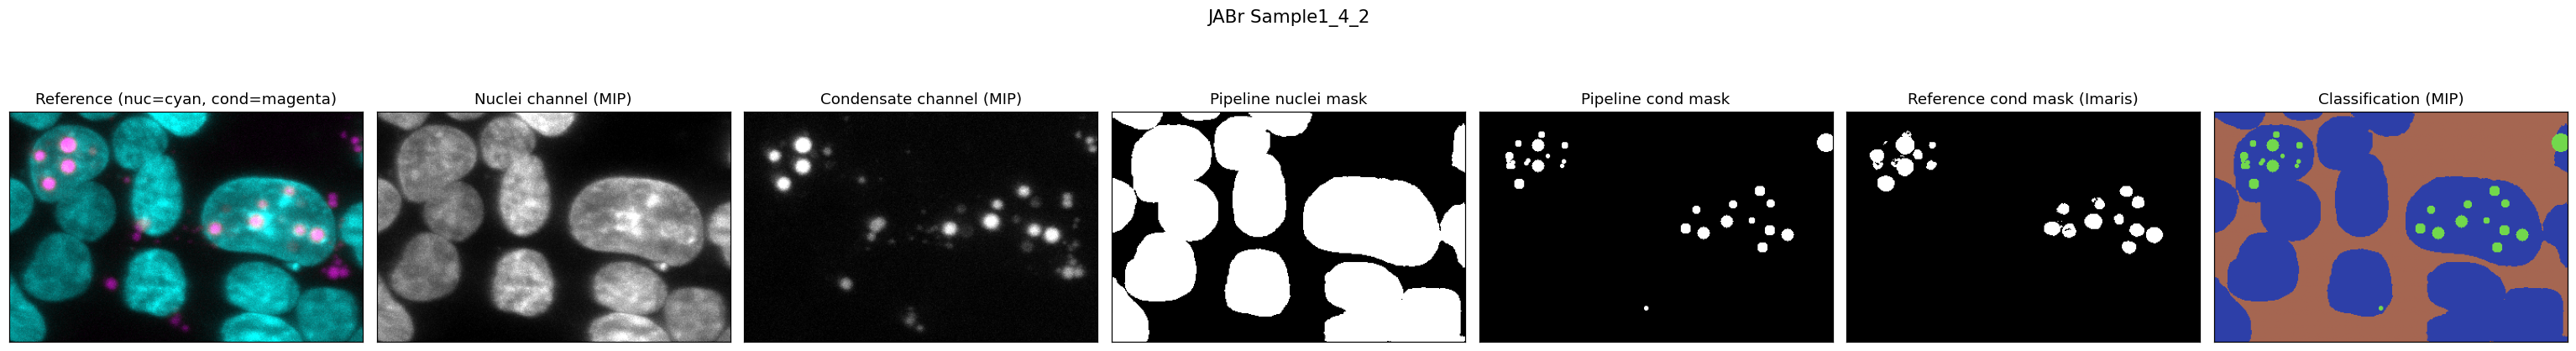
\includegraphics[width=\textwidth]{Sample1_4_2.png}\\
{\small Sample1\_4\_2 --- best case: ref PC 5.05, calibrated 5.06, err 0.3\%}
\end{center}
\vspace{0.4em}
\begin{center}
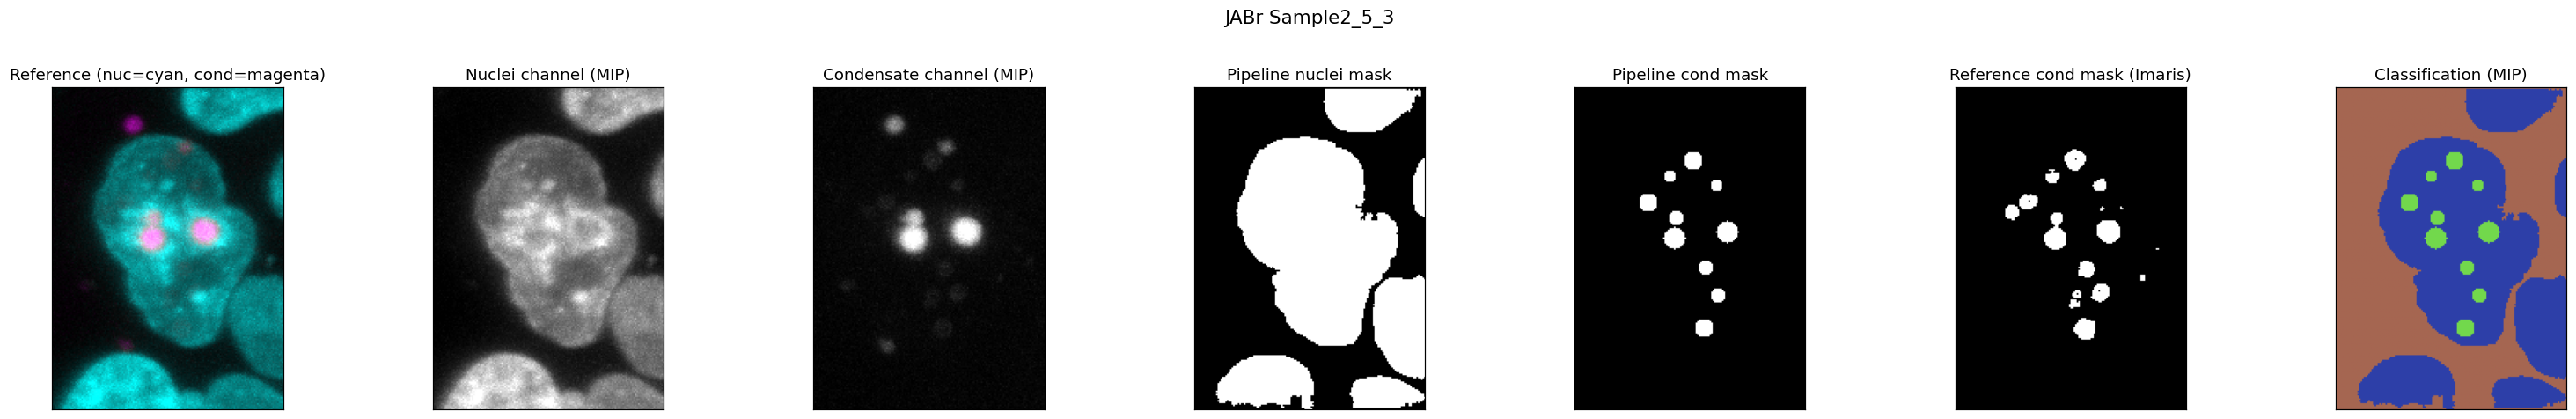
\includegraphics[width=\textwidth]{Sample2_5_3.png}\\
{\small Sample2\_5\_3 --- bundled sample: ref PC 4.56, calibrated 4.67, err 2.4\%}
\end{center}
\vspace{0.4em}
\begin{center}
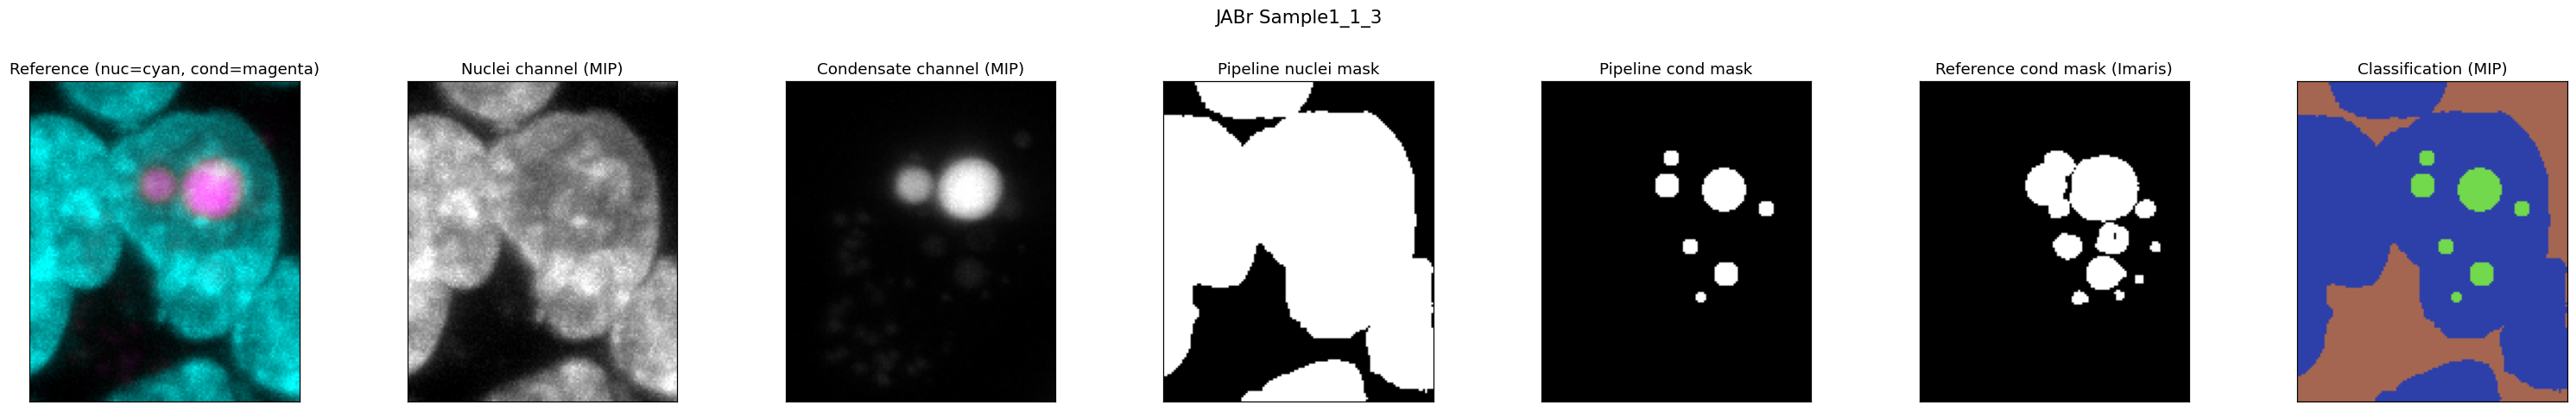
\includegraphics[width=\textwidth]{Sample1_1_3.png}\\
{\small Sample1\_1\_3 --- high PC: ref 19.77, calibrated 19.53, err 1.2\%}
\end{center}
\vspace{0.4em}
\begin{center}
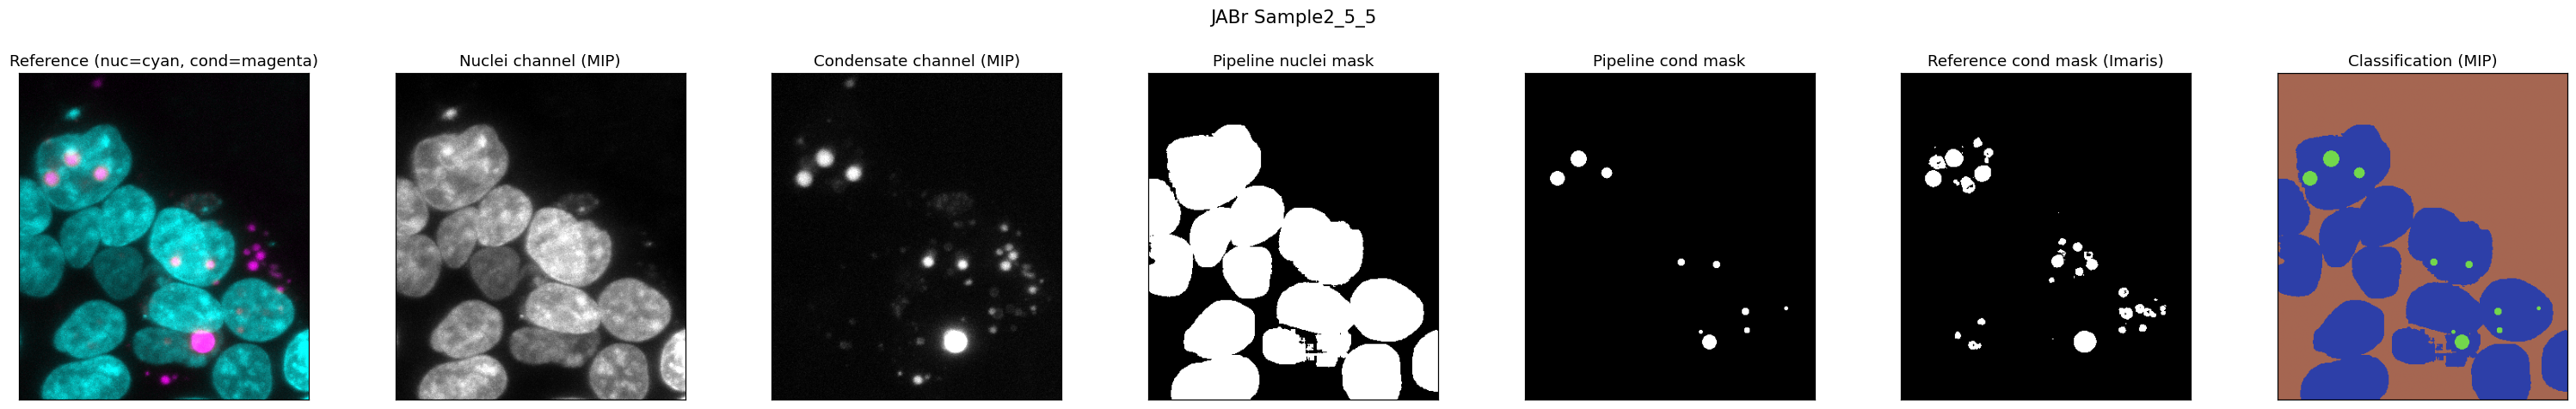
\includegraphics[width=\textwidth]{Sample2_5_5.png}\\
{\small Sample2\_5\_5 --- rescued by the sphere-overlap gate: was $+58\%$, now ref 6.73 / calibrated 5.72, err 15\%}
\end{center}
\vspace{0.4em}
\begin{center}
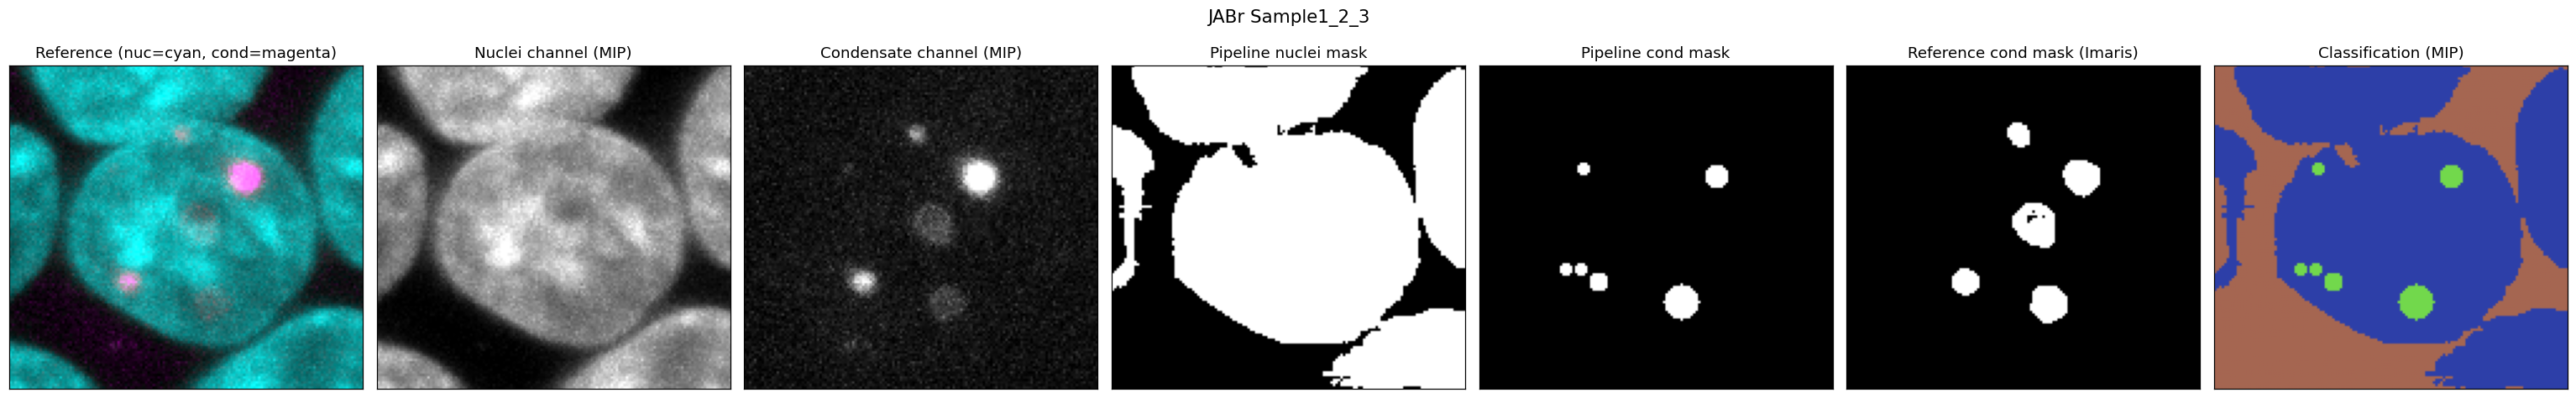
\includegraphics[width=\textwidth]{Sample1_2_3.png}\\
{\small Sample1\_2\_3 --- failure: ref 2.55, calibrated 4.15, err 63\% (calibration-floor effect)}
\end{center}
\vspace{0.4em}
\begin{center}
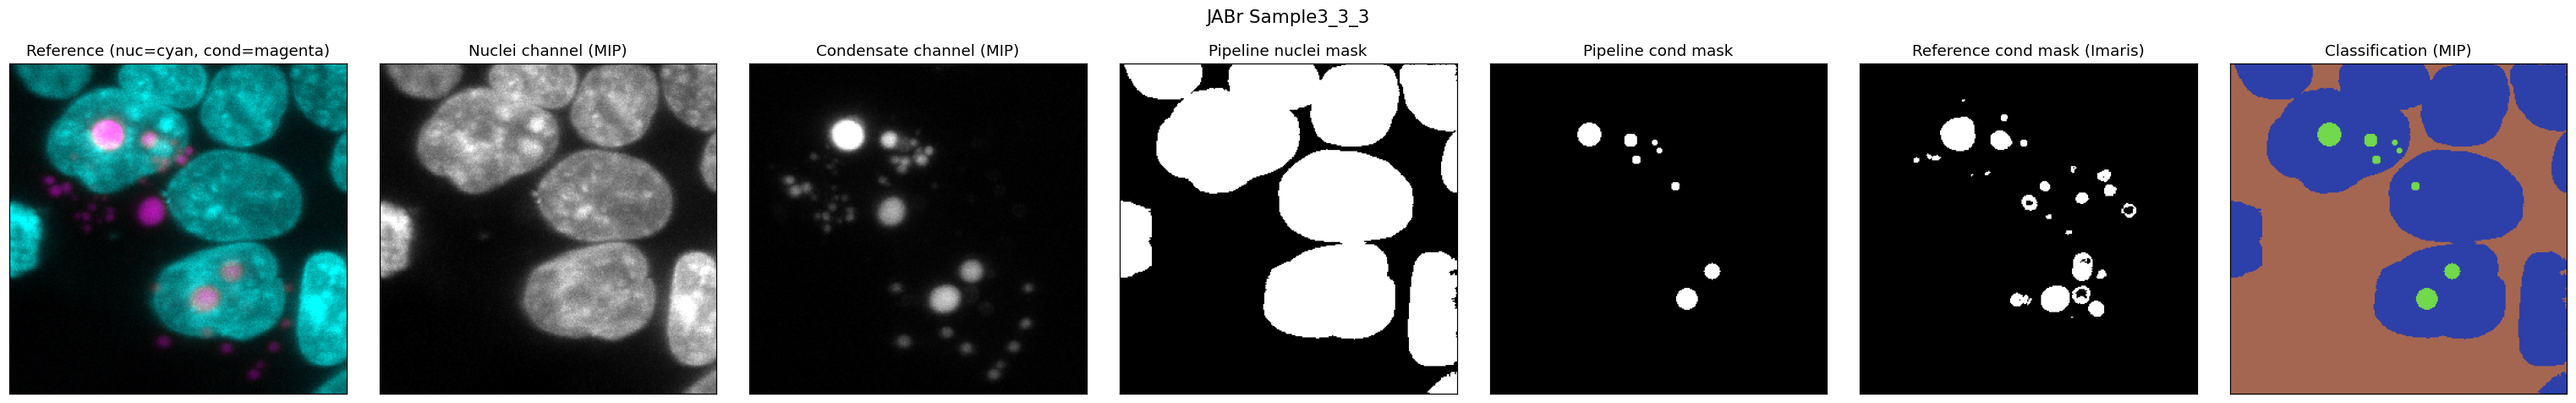
\includegraphics[width=\textwidth]{Sample3_3_3.png}\\
{\small Sample3\_3\_3 --- failure: ref 8.82, calibrated 11.42, err 29\% (over-bright blobs)}
\end{center}
\vspace{0.4em}
\end{document}